\documentclass[onecolumn]{article}
%\usepackage{url}
%\usepackage{algorithmic}
\usepackage[a4paper]{geometry}
\usepackage{datetime}
\usepackage[margin=2em, font=small,labelfont=it]{caption}
\usepackage{graphicx}
\usepackage{mathpazo} % use palatino
\usepackage[scaled]{helvet} % helvetica
\usepackage{microtype}
\usepackage{amsmath}
\usepackage{amsthm}
\usepackage{xcolor}
\usepackage{subfigure}
\usepackage{optidef}
\usepackage{float}
\usepackage{tikz}
\DeclareUnicodeCharacter{2212}{\ensuremath{-}}
\usetikzlibrary{patterns}  

% Letterspacing macros
\newcommand{\spacecaps}[1]{\textls[200]{\MakeUppercase{#1}}}
\newcommand{\spacesc}[1]{\textls[50]{\textsc{\MakeLowercase{#1}}}}

\title{\spacecaps{Exercise 1: Convex Sets}\\ \normalsize \spacesc{31099/61099, Applied Optimization } }

\author{Colmenar Herrera Marta\\Wu Shunyu\\Hamedi Zahra}
%\date{\today\\\currenttime}
\date{\today}

\begin{document}
\maketitle
% \textcolor{red}{(REVIEW THE NUMBER OF THE EQUATIONS BEFORE SUBMITTING)}

\section{Example sets (2 pt)}
\textcolor{teal}{\emph{Sketch the following sets in R2}}
\subsection{ $\text{span}\left\{\binom{1}{1}, \binom{-0.5}{-0.5} \right\}$}
\begin{figure}[H]
    \center
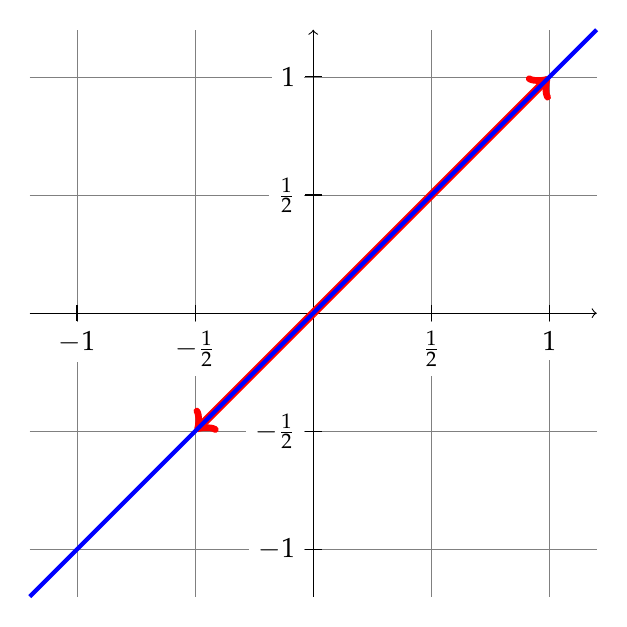
\begin{tikzpicture}[scale=3]
 \draw[step=.5cm, gray, very thin] (-1.2,-1.2) grid (1.2,1.2); 
  \draw[->] (-1.2,0) -- (1.2,0) coordinate (x axis);
  \draw[->] (0,-1.2) -- (0,1.2) coordinate (y axis);
  \draw[->, line width=3pt, color=red] (0,0) -- (1,1);
  \draw[->, line width=3pt, color=red] (0,0) -- (-0.5,-0.5);
  \draw [blue, line width=1.5pt, domain=-1.2:1.2] plot (\x, \x); 
  \foreach \x/\xtext in {-1, -0.5/-\frac{1}{2}, 0.5/\frac{1}{2}, 1} 
   \draw (\x cm,1pt) -- (\x cm,-1pt) node[anchor=north,fill=white] {$\xtext$};
 \foreach \y/\ytext in {-1, -0.5/-\frac{1}{2}, 0.5/\frac{1}{2}, 1} 
   \draw (1pt,\y cm) -- (-1pt,\y cm) node[anchor=east,fill=white] {$\ytext$};
\end{tikzpicture}
\end{figure}

\subsection{ $\text{span}\left\{\binom{1}{1}, \binom{0.5}{-0.5} \right\}$}
\begin{figure}[H]
    \center
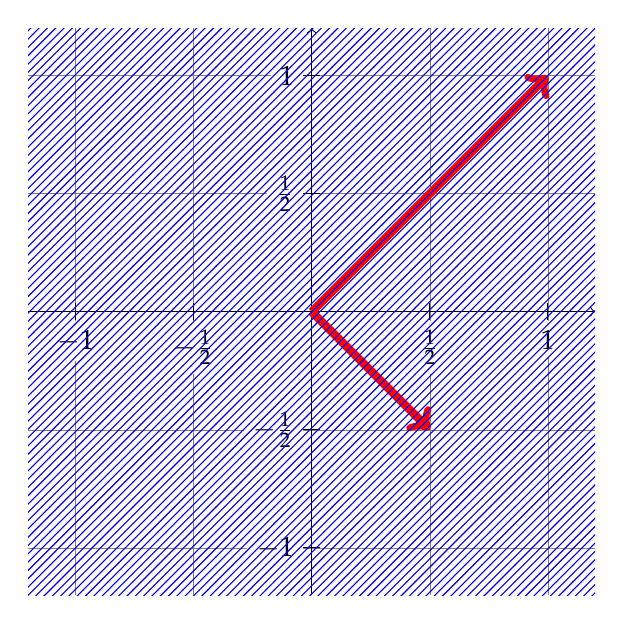
\begin{tikzpicture}[scale=3]
 \draw[step=.5cm, gray, very thin] (-1.2,-1.2) grid (1.2,1.2); 
  \draw[->] (-1.2,0) -- (1.2,0) coordinate (x axis);
  \draw[->] (0,-1.2) -- (0,1.2) coordinate (y axis);
  \draw[->, line width=3pt, color=red] (0,0) -- (1,1);
  \draw[->, line width=3pt, color=red] (0,0) -- (0.5,-0.5);
  \foreach \x/\xtext in {-1, -0.5/-\frac{1}{2}, 0.5/\frac{1}{2}, 1} 
   \draw (\x cm,1pt) -- (\x cm,-1pt) node[anchor=north,fill=white] {$\xtext$};
 \foreach \y/\ytext in {-1, -0.5/-\frac{1}{2}, 0.5/\frac{1}{2}, 1} 
   \draw (1pt,\y cm) -- (-1pt,\y cm) node[anchor=east,fill=white] {$\ytext$};
   \fill[pattern=north east lines, pattern color=blue,fill opacity=0.3] (-1.2,-1.2) rectangle (1.2,1.2);
\end{tikzpicture}
\end{figure}


\subsection{ $\text{aff}\left\{\binom{1}{0}, \binom{1}{-1} \right\}$}
\begin{figure}[H]
    \center
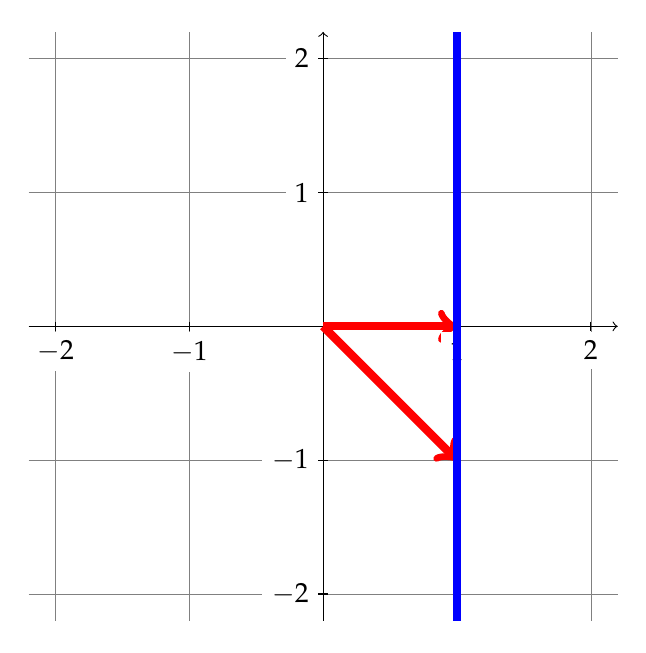
\begin{tikzpicture}[scale=1.7]
 \draw[step=1cm, gray, very thin] (-2.2,-2.2) grid (2.2,2.2); 
  \draw[->] (-2.2,0) -- (2.2,0) coordinate (x axis);
  \draw[->] (0,-2.2) -- (0,2.2) coordinate (y axis);
  \draw[->, line width=3pt, color=red] (0,0) -- (1,0);
  \draw[->, line width=3pt, color=red] (0,0) -- (1,-1);
  \foreach \x/\xtext in {-2, -1, 1, 2} 
   \draw (\x cm,1pt) -- (\x cm,-1pt) node[anchor=north,fill=white] {$\xtext$};
 \foreach \y/\ytext in {-2, -1, 1, 2} 
   \draw (1pt,\y cm) -- (-1pt,\y cm) node[anchor=east,fill=white] {$\ytext$};
 \draw[color=blue,line width=3pt] (1,-2.2) -- (1,2.2);
\end{tikzpicture}
\end{figure}

\subsection{$\text{conv}\left\{\binom{1}{0}, \binom{2}{1}, \binom{3}{-2}, \binom{-1}{0}, \binom{-2}{1}, \binom{-2}{-2} \right\}$}
\begin{figure}[H]
    \center
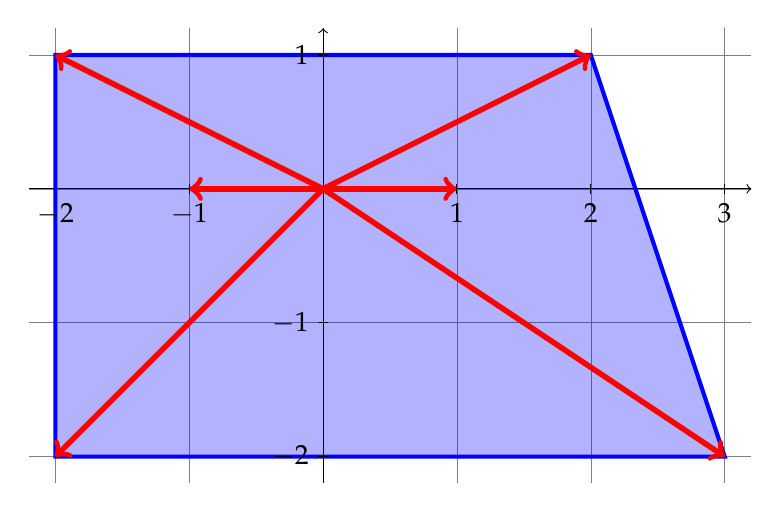
\begin{tikzpicture}[scale=1.7]
 \draw[step=1cm, gray, very thin] (-2.2,-2.2) grid (3.2,1.2); 
  \draw[->] (-2.2,0) -- (3.2,0) coordinate (x axis);
  \draw[->] (0,-2.2) -- (0,1.2) coordinate (y axis);
  
  \draw[pattern=north east lines, pattern color=blue, color=blue, fill opacity=0.3,line width=1.5pt]
        (2,1) --
        (3,-2) --
        (-2,-2) --
        (-2,1) --
        cycle;

    \draw[->, line width=2pt, color=red] (0,0) -- (1,0);
    \draw[->, line width=2pt, color=red] (0,0) -- (2,1);
    \draw[->, line width=2pt, color=red] (0,0) -- (3,-2);
    \draw[->, line width=2pt, color=red] (0,0) -- (-1,0);
    \draw[->, line width=2pt, color=red] (0,0) -- (-2,1);
    \draw[->, line width=2pt, color=red] (0,0) -- (-2,-2);

  \foreach \x/\xtext in {-2, -1, 1, 2, 3} 
   \draw (\x cm,1pt) -- (\x cm,-1pt) node[anchor=north] {$\xtext$};
 \foreach \y/\ytext in {-2, -1, 1} 
   \draw (1pt,\y cm) -- (-1pt,\y cm) node[anchor=east] {$\ytext$};

\end{tikzpicture}
\end{figure}


\section{Convexity (1 pt)}

\textcolor{teal}{\emph{Let $C \in \mathbb{R}^n $ be a convex set, with $x_1,...,x_k \in C$, and let $\theta_1,...,\theta_k \in \mathbb{R}$ satisfy $\theta_i \ge 0$, $\theta_1 + ... + \theta_k = 1$. Show that $\theta_1 x_1 + ... + \theta_k x_k \in C$.}}
\begin{proof}
When $k=1$, this says that each point of $C$ is a point of $C$. When $k=2$, it means whenever $\theta_1 + \theta_2 = 1$ the point $\theta_1 x_1 + \theta_2 x_2$ is in $C$ because $\theta_2 = 1 - \theta_1$ and so the point in question is $\theta_1 x_1 + (1-\theta_1) x_2$, which is a point on the line between $x_1$ and $x_2$. 

Now we assume all length-$(k-1)$ combinations are contained in $C$, and take a length-$k$ combination of points in $C$:
\[\theta_1 x_1 + \theta_2 x_2 + ... + \theta_k x_k\]
By the inductive hypothesis, we know that 
\[ y = \frac{\theta_1}{\theta_1 + \theta_2 + ... + \theta_{k-1}} x_1 + \frac{\theta_2}{\theta_1 + \theta_2 + ... + \theta_{k-1}} x_2 + ... + \frac{\theta_{k-1}}{\theta_1 + \theta_2 + ... + \theta_{k-1}} x_{k-1}\]
is in $C$. (This is only defined if $\theta_1 + ... + \theta_{k-1} \neq 0$; if it's $0$, then $\theta_k$ is the only nonzero coefficient, so we effectively had a length-1 convex combination to begin with.) If not, the original convex combination can be written as 
\[\theta_1 x_1 + \theta_2 x_2 + ... + \theta_k x_k = (\theta_1 + ... + \theta_{k-1})y + \theta_k x_k\]
which lies on the line segment $[y,x_k]$, and therefore it is in $C$ by the definition of a convex set. Therefore by induction, convex combinations of all size must be contained in $C$.

\end{proof}


\section{Linear Equations (1 pt)}
\textcolor{teal}{\emph{Show that the solution set of linear equations $\{x | Ax = b\}$ with $x \in \mathbb{R}^n$, $A \in \mathbb{R}^{mxn}$ and $b \in \mathbb{R}^m$ is an affine set.}}

We choose two elements from set:  $x_0, x_1$ 
\[x_0 , x_1 \in R^n\]
\[A x_0 = b\]
\[A x_1 = b\]
Affine set \textrightarrow \; $\alpha A x_0 + (1-\alpha) A x_1= \alpha A x_0 +A x_1-\alpha A x_1 = \alpha b + b - \alpha b = b$ 
\\
So, the affine combination is also a solution.



\section{Linear Inequations (1 pt)}
\textcolor{teal}{\emph{1. Show that the solution set of linear inequations $\{x | Ax \preceq b, Cx = d\}$ with $x \in \mathbb{R}^n$, $A \in \mathbb{R}^{mxn}$ and $b \in \mathbb{R}^m$, $C \in \mathbb{R}^{kxn}$ and $d \in \mathbb{R}^k$ is a convex set. Here $\preceq$ means componentwise less or equal. }}

We choose two elements from set:  $x_0, x_1$ 
\[A x_0 \preceq b\]
\[A x_1 \preceq b\]
\[\alpha , \beta \geq 0\]
\[\alpha + \beta = 1 \xrightarrow{ } \alpha = 1- \beta \geq 0  \xrightarrow{} \beta \leq 1\]
\[ \beta \in [0,1] \]

\[\alpha A x_0 + \beta A x_1= (1-\beta) A x_0 + \beta A x_1 \] 
because $ \; A x_0 \preceq b\ and \; A x_1 \preceq b $ and also $ \beta \in [0,1] $
\\
We can conclude that this equation is also less than b:
\[(1-\beta) A x_0 + \beta A x_1 \preceq  (1-\beta) b + \beta b\] 
\[(1-\beta) A x_0 + \beta A x_1 \preceq  b\] 
Also:
\[C x_0 = d\]
\[C x_1 = d\]
\[ (1-\beta)C x_0 +\beta C x_1 = C x_0 - \beta C x_0 +\beta C x_1 = d - \beta d +\beta d = d\]
\\
\textcolor{teal}{\emph{2. Is it an affine set?}}
\[C x_0 = d\]
\[C x_1 = d\]
\[ (1-\beta)C x_0 +\beta C x_1 = C x_0 - \beta C x_0 +\beta C x_1 = d - \beta d +\beta d = d\]
to check $A x \preceq b$ :
\[A x_0 \preceq b\]
\[A x_1 \preceq b\]
\[\alpha A x_0 + (1-\alpha)A x_1\]
We have $ \; A x_0 \preceq b\ and \; A x_1 \preceq b $ but this time $\alpha \in R $ so, we do not have any limits for $\alpha$ and we cannot conclude that $\alpha A x_0 + (1-\alpha) A x_1 \preceq  b $
\\
So, it's not affine.


\section{Voronoi description of halfspace (1 pt)}
\textcolor{teal}{\emph{Let $a$ and $b$ be distinct points in $\mathbb{R}^n$. Show that the set of all points that are closer (in Euclidean norm) to $a$ than $b$, i.e., $\{x | \left\lVert x − a\right\rVert ^2 \le \left\lVert x − b\right\rVert ^2\}$, is a halfspace. Describe it explicitly as an inequality of the form $c^T x \le d$. Draw a picture.}}

Let $a$ and $b$ be distinct points in $\mathbb{R}$. We need to show that the set of all points that are closer (in Euclidean norm) to $a$ than $b$, i.e., $\{x \mid \lVert x − a \rVert ^2 \leq \lVert x − b \rVert ^2 \}$, is a halfspace. \hfill \break 
To describe it as an inequality of the form $c^T x \leq d$, we are going to start resolving the inequality $\lVert x − a \rVert ^2 \leq \lVert x − b \rVert ^2$ as follows 

\begin{equation*}
    \lVert x − a \rVert ^2 \leq \lVert x − b \rVert ^2
\end{equation*}
\begin{equation*}
    (x-a)(x-a)^T \leq (x-b)(x-b)^T 
\end{equation*}  \hfill \break

Solving $(x-a)(x-a)^T$ and similarly $(x-b)(x-b)^T$, we get
\begin{equation*}
    (x-a)(x-a)^T = x^2 - xa^T -ax^T + a^2 = x^2 -2a^Tx + a^2
\end{equation*}
\begin{equation*}
    x^2 -2a^Tx + a^2 \leq x^2 -2b^Tx + b^2
\end{equation*}
\begin{equation}\label{eq:final}
    a^2 -2a^Tx \leq b^2 -2b^Tx 
\end{equation}  \hfill \break

Rewriting the inequality \ref{eq:final} as, $2(b^T - a^T)x \leq b^2 - a^2$. We get the expression we were looking for, where $c^T = 2(b^T - a^T)$ and $d = b^2 - a^2$.
\begin{figure}[H]
    \center
    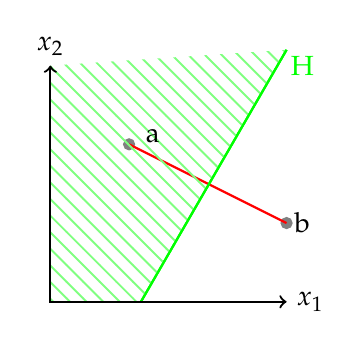
\begin{tikzpicture}
        \pgfdeclarepatternformonly{north east lines wide}%
        {\pgfqpoint{-1pt}{-1pt}}%
        {\pgfqpoint{10pt}{10pt}}%
        {\pgfqpoint{9pt}{9pt}}%
        {
        \pgfsetlinewidth{0.7pt}
        \pgfpathmoveto{\pgfqpoint{0pt}{0pt}}
        \pgfpathlineto{\pgfqpoint{9.1pt}{9.1pt}}
        \pgfusepath{stroke}
        }
    
        \pgfdeclarepatternformonly{north west lines wide}
        {\pgfqpoint{-1pt}{-1pt}}%
        {\pgfqpoint{7pt}{7pt}}%
        {\pgfqpoint{6pt}{6pt}}%
        {
        \pgfsetlinewidth{0.7pt}
        \pgfpathmoveto{\pgfqpoint{0pt}{6pt}}
        \pgfpathlineto{\pgfqpoint{6.1pt}{-0.1pt}}
        \pgfusepath{stroke}
        }
    
        \filldraw[color=gray] (1,2) circle (2pt); 
        \filldraw[color=gray] (3,1) circle (2pt); 
        
        % Draw two intersecting lines
        \draw[thick, red]   (1,2) coordinate (a) -- (3,1) coordinate (b);
        \draw[thick, green] ( 3,3.2) coordinate (c) -- (1.15, 0) coordinate (d);
    
        \fill[pattern=north west lines wide, pattern color=green!50] (1.15, 0) -- (0,0) -- (0,3) -- (3,3.2)--(2,1.5);
    
        \draw[thick, green] (c) -- (d);
    
        % Draw axes
        \draw [<->,thick] (0,3) node (yaxis) [above] {$x_2$}
            |- (3,0) node (xaxis) [right] {$x_1$};
        \node[green]   at (3.2,3) {H};
        \node[black]   at (1.3,2.1) {a};
        \node[black]   at (3.2,1) {b};
    \end{tikzpicture}
\end{figure}  

\section{Convex Illumination Problem (3 pts)}

Show that the solution $p^* = (p_{1}^*, p_{2}^*,..., p_{n}^*)^T \in \mathbb{R}^n$ of the non-convex illumination problem
from the lecture
\begin{mini!}|l|
    {}{\max\limits_{k = 1...m} \mid log I_k - log I_{des} \mid}
    {}{}
    \addConstraint{0 \leq p_j \leq p_{max}, j = 1...n}
\end{mini!}
\nocite{*}
with $I_k = \sum_{j=1}^{n} a_{kj}p_j$ for geometric constants $a_{jk} \in \mathbb{R}$, a constant desired ilumination $i_{des} \in \mathbb{R}$ and a upper bound $p_{max} \in \mathbb{R}$ on the lamp power, is identical to the solution of the following equivalent (convex) problem
\begin{mini!}|l|
    {}{\max\limits_{k = 1...m} h(I_k / I_{des})}
    {}{}
    \addConstraint{0 \leq p_j \leq p_{max}, j = 1...n}
\end{mini!}
\nocite{*}
with $h(u) = \max \{u, 1/u\}.$ \hfill \break
\begin{proof}


To prove that solving the optimization problem (2a) is equal to solving (3a), we are going to transform the maximum expression (3a) into the maximum expression (2a).\\
Taking $h(u) = \max \{u, 1/u\}$, and $u = I_k / I_{des}$, it is possible to rewrite the expression (3a) as
\begin{equation*}
    h(I_k / I_{des}) = \max \{ I_k / I_{des}, I_{des} / I_k \}
\end{equation*}
Knowing that the maximum value of the convex function $ h(I_k / I_{des})$ is not going to change if we take its logarithm. And, that $\log(a/b) = \log(a) - \log(b)$. We obtain
\begin{align*}
     \log (\max_{k=1,...,m} h(I_k / I_{des})) 
     & = \log (\max_{k=1,...,m} \max \{ I_k / I_{des}, I_{des} / I_k \}) \\
     & = \max_{k=1,...,m} \max \{ \log(I_k / I_{des}), \log(I_{des} / I_k) \} \\
    & = \max_{k=1,...,m} \{ \log(I_k) - \log(I_{des}), \log(I_{des}) - \log(I_k) \} \stepcounter{equation}\tag{\theequation}\label{eq:max_log}
\end{align*} \hfill \break

If we call the $\log(I_k) - \log(I_{des})$ as A in the expression \ref{eq:max_log}. We can clearly see that has the shape of $\max \{A, -A\}$, what we can rewrite as $\max \mid A\mid$. Our expression will be
\begin{equation*}
    \max_{k=1,...,m}  \mid \log(I_k) - \log(I_{des}) \mid
\end{equation*}
Being demonstrated that solving the non-convex ilumination problem, is identical to the solution of equivalent convex problem.
\end{proof}

\bibliographystyle{plain}
\bibliography{references}
\end{document}

